%--------------------------------------------------------------------------------------------------
\chapter{Aufbau des Konzepts}\label{cha:AufbauDesKonzepts}

In diesem Kapitel wird der Aufbau des Konzepts erklärt. Daher gibt es zu erst einen Einblick in den Digitalisierungsprozess von Produktionseinlagen. Daraufhin wird diese Arbeit in das Gesamtkonzept der Mensch-Maschine Interaktion eingeordnet. Schließlich wird der Aufbau des Modells mithilfe des Functional-Mockup Interfaces erklärt.

%--------------------------------------------------------------------------------------------------
\section{Von der physischen Produktionsanlage zum virtuellen Klon}\label{sec:PhysischZumKlon}

Um die Produktionsabläufe einer Fabrik in einer virtuellen Welt abzubilden gibt es insgesamt sieben Schritte die befolgt werden müssen.

\begin{enumerate}
	\item \textbf{Scannen der Fabrik} \\
	Im ersten Schritt werden die Produktionsräume inklusive der Produktionsanlagen gescannt. Das Ergebnis dieses Scans ist eine Punktwolke.
	\item \textbf{Umwandlung des Scans} \\
	Der Scan muss von einer Punktewolke in CAD Modelle umgewandelt werden. Da die CAD Modelle zu groß und daher unpraktikabel für die Entwicklungsumgebung Unity sind, werden diese in das OBJ Format umgewandelt. Die Modelle sind für den späteren Aufbau des virtuellen Klons der echten Produktionsanlage notwendig.
	\item \textbf{Abbildung: Produktionsanlage $\rightarrow$ Modell} \\
	Es wird ein physisches Modell zur Darstellung einiger wichtiger Herausforderungen der echten Produktionsanlage gebaut. Dies könnte Beispielsweise die Form einer Produktionsstraße mit mehreren Stationen besitzen.
	\item \textbf{Virtueller Aufbau} \\
	Das physische Modell der echten Produktionsanlage aus Schritt drei wird in der virtuellen Welt abgebildet (virtueller Klon) und mit dem Menschmodell begehbar gemacht. Dieser Schritt erlaubt die virtuelle Planung einer Produktionsanlage.
	\item \textbf{Konnektivität und Kommunikation} \\
	Die Produktionsanlagen des physischen Modells werden mit der Cloud vernetzt um eine bidirektionale Kommunikation zwischen dem physischem Modell und dem virtuellen Klon zu ermöglichen.
	\item \textbf{Interaktion} \\
	Die Interaktion mit zwischen dem Bediener und den Produktionsanlagen in der virtuellen Welt wird implementiert. Es müssen unter Umständen anwendungsspezifische Benutzeroberflächen implementiert werden.
	\item \textbf{Skalierung} \\
	Skalierung der Vorgehensweise durch Anwendung von Schritt vier bis sechs auf die echte Produktionsanlage.
\end{enumerate}
Durch das Einhalten dieser Schritte erhält man einen virtuellen Klon der echten Produktionsanlage. Diesen virtuellen Klon kann man für viele Zwecke einsetzen, dazu gehören Beispielsweise die Produktionsplanung oder das Fernsteuern von Produktionsanlagen. Das Ergebnis dieser Arbeit kommt bei Schritt vier und sechs zum Einsatz [Quelle Yübo?].

%--------------------------------------------------------------------------------------------------
\section{Mensch-Maschine Interaktion im Kontext dieser Arbeit}\label{sec:MMInteraktion}
\begin{figure}[h]
	\centering
	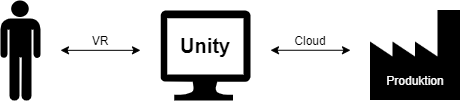
\includegraphics[width=0.7\linewidth]{Bilder/A19_MMI}
	\caption{Mensch-Maschine Interaktion im Kontext dieser Arbeit, eigene Abbildung}
	\label{fig:A}
\end{figure}
\noindent Durch die Abbildung der echten Produktionsanlage in der virtuellen Welt findet die Mensch-Maschine-Interaktion in zwei Schritten statt. Im ersten Schritt interagiert der Mensch mit der Software (dem Computer) über VR-Hardware. Dieser Computer interagiert dann über eine Cloud mit der echten Produktionsanlage. Die Kommunikation findet in beiden Schritten bidirektional statt.
\newline\newline
Diese Arbeit befasst sich mit dem ersten Schritt der oben erklärten Mensch-Maschine Interaktion. Für dem Rest dieser Arbeit werden wir annehmen, dass es bereits eine geeignete Infrastruktur für die Kommunikation zwischen dem Computer und der Produktionsanlage über eine Cloud gibt.

%--------------------------------------------------------------------------------------------------